% !TeX program = xelatex
% !TeX encoding = UTF-8
% 在实验三根目录运行 XeLaTeX 两次，以更新目录和交叉引用。
\documentclass[UTF8,zihao=-4,fontset=windows]{ctexart}
\usepackage[a4paper,left=20mm,right=20mm,top=16mm,bottom=16mm,
  includeheadfoot,headheight=15pt,headsep=5mm,footskip=9mm]{geometry}
\usepackage{graphicx,booktabs,array,tabularx,xcolor,fancyhdr}
\usepackage[unicode,hidelinks]{hyperref}

\definecolor{reportnavy}{HTML}{192A44}
\definecolor{reportgray}{HTML}{506177}
\ctexset{
  section = {format = \Large\bfseries\raggedright\color{reportnavy}},
  subsection = {format = \large\bfseries\raggedright\color{reportnavy}}
}
\hypersetup{
  pdftitle={软件工程实验三报告},
  pdfauthor={张博睿},
  pdfsubject={学校来宾酒店预订系统的代码实现与验证},
  bookmarksnumbered=true
}
\setlength{\parskip}{0.35em}
\setlength{\parindent}{2em}
\setlength{\emergencystretch}{1.5em}
\setcounter{tocdepth}{1}
\renewcommand{\arraystretch}{1.22}
\newcolumntype{Y}{>{\raggedright\arraybackslash}X}
\renewcommand{\headrulewidth}{0.35pt}
\pagestyle{fancy}
\fancyhf{}
\fancyhead[L]{\small\color{reportgray}软件工程实验三}
\fancyhead[R]{\small\color{reportgray}学宾接待}
\fancyfoot[C]{\small\color{reportgray}\thepage}

\begin{document}

\thispagestyle{empty}
\vspace*{31mm}
\begin{center}
  {\color{reportnavy}\zihao{1}\bfseries 软件工程实验三报告\par}
  \vspace{6mm}
  {\color{reportgray}\zihao{3}学宾接待 · 学校来宾酒店预订系统\par}
  \vspace{15mm}
  \begin{tabular}{@{}r@{\qquad}l@{}}
    姓名 & 张博睿 \\
    学号 & 241220007 \\
    日期 & 2026年11月24日 \\
  \end{tabular}
\end{center}
\vspace{15mm}

\noindent\textbf{实验内容}\par
依据实验二的需求、UML 模型和界面原型实现住宿预订系统。系统面向学校接待人员、酒店工作人员、平台管理员和来宾，覆盖酒店查询、自动预订、到店退房及停业安置。本次实验交付可在 Windows 本地运行的桌面程序，并核对关键业务规则与运行结果。

\vspace{7mm}
\tableofcontents

\clearpage

\section{根据 UML 图实现代码}
\subsection{模型到代码的转换}

实现时先用用例图确定四类角色的操作范围，再按组件图分配后端职责。桌面窗口由 WinForms 和 WebView2 承载，Vue 页面通过本机 HTTP 接口与 Spring Boot 后端通信。后端保留十个逻辑模块，由统一的接口层接收请求，使用 JDBC 和同一个数据库完成业务写入。

{\small
\noindent\begin{tabularx}{\linewidth}{@{}p{25mm}p{57mm}Y@{}}
\toprule
\textbf{UML 图} & \textbf{模型中的内容} & \textbf{实现中的对应关系} \\
\midrule
用例图 & 四类用户的业务入口和责任范围 &
\path{App.vue} 按角色呈现工作区，\path{SecurityConfig} 和 \path{Access} 校验身份、接待责任、酒店归属及来宾本人范围。 \\
组件图 & 查询、订单、履约、安置和支撑模块间的依赖 &
\path{ApiController} 接入请求，\path{SearchService}、\path{BookingService}、\path{StayService} 和 \path{RelocationService} 分担业务职责。 \\
类图 & 住宿需求、房型、逐日房源、订单及逐晚明细 &
以 \path{Plan} 表示住宿条件。订单和明细分别落入 \path{booking_order}、\path{order_item}、\path{order_night}，按订单及明细编号关联。 \\
状态图 & 预订、入住、退房、取消、未入住和停业安置 &
\path{OrderState.transitionTo} 定义状态迁移，预订与履约服务统一调用状态校验。 \\
自动预订序列图 & 权限检查、请求查重、方案复核和整单提交 &
\path{CommandService} 保存处理结果，\path{BookingService} 与房源模块在事务内复核并确认预订。 \\
停业安置序列图 & 停售、保留占用、通知和确认替代新单 &
\path{RelocationService} 维护安置记录，\path{NotificationService} 生成站内通知和邮件任务。 \\
\bottomrule
\end{tabularx}\par
}

在数据层，\path{daily_inventory} 对“酒店、房型、住宿日期”设置联合唯一约束，可用量按学校名额减去占用和维修扣减计算。计划住宿写入逐晚预订明细，到店按来宾登记，实际间夜按房间明细及日期登记。三类记录分别支撑报价、履约和实际住宿统计。

当前接待界面选择一种房型并填写间数，查询时同时校验来宾容量、每晚价格区间、整单预算和距离。后端依照类图使用房型明细列表，集成测试覆盖同一订单多个明细的全量提交和失败回滚。

\clearpage

\subsection{关键流程与状态约束}

\textbf{自动预订}。接待人员确认报价和规则后提交本次方案及请求标识。\path{CommandService} 在请求表中查重并返回已有结果。新请求由 \path{BookingService} 复核报价和各晚名额。方案仍合格但价格、名额或规则已变时，页面提示重新确认。任一晚不足则整单失败。成功时，事务一并保存订单、逐晚锁定价、规则快照、名额占用和请求结果。

\textbf{状态迁移}。首位来宾登记后，已确认订单转为已入住。同单后来宾补登记沿用该状态。退房时保存实际住宿并释放未住日期的名额。订单状态与请求处理结果分别记录。确认新方案使用新的请求标识，原请求结果仍可查询。

\textbf{停业安置}。确认停业影响范围后，系统标记停售并暂留原单占用。接待人员确认替代方案且新单成功后，系统在同一事务内关联新单、关闭原单并释放原占用。已住间夜和费用保留在原单，通知发送结果独立跟进。

\begin{figure}[!ht]
  \centering
  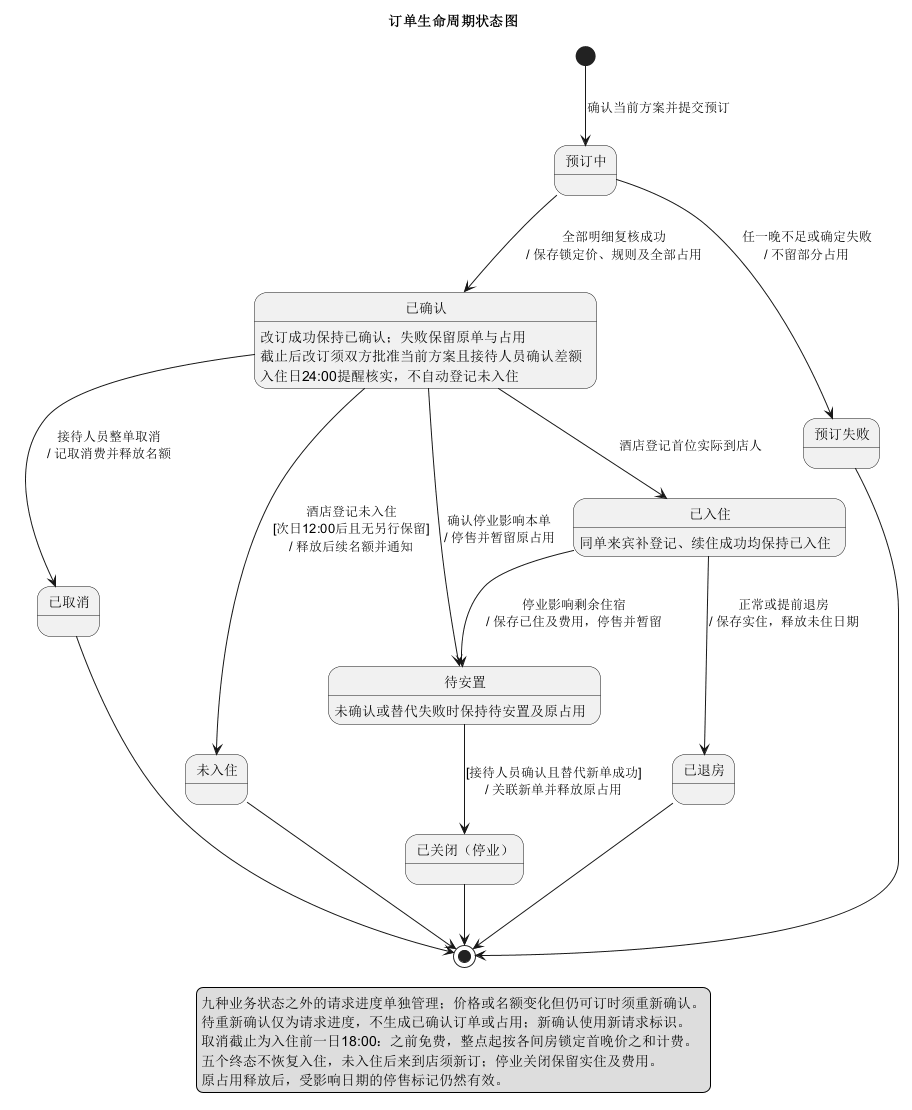
\includegraphics[width=\linewidth,height=139mm,keepaspectratio]{uml/UML状态图.png}
  \caption{订单生命周期状态图，迁移关系对应 \texttt{OrderState}}
  \label{fig:order-state}
\end{figure}

\clearpage

\subsection{源代码规模}

对 \path{code/} 中的自编程序源码、数据库迁移、构建启动脚本和测试源码逐文件计数。主程序与数据库迁移共 58 个文件、6,792 行。计入构建启动脚本及测试后，共 71 个文件、8,624 行。

\vspace{3mm}
{\small
\noindent\begin{tabularx}{\linewidth}{@{}Yrr@{}}
\toprule
\textbf{统计范围} & \textbf{文件数} & \textbf{物理行数} \\
\midrule
后端主程序 Java & 30 & 5,632 \\
前端 Vue、TypeScript、CSS 和入口 HTML & 24 & 728 \\
Windows 桌面入口 C\# & 1 & 265 \\
数据库迁移 SQL & 3 & 167 \\
构建和启动脚本 PowerShell、CMD、JavaScript & 8 & 221 \\
后端集成与迁移测试 Java & 2 & 1,202 \\
前端操作测试 TypeScript & 3 & 409 \\
\midrule
\textbf{合计} & \textbf{71} & \textbf{8,624} \\
\bottomrule
\end{tabularx}\par
}

\subsection{你是怎么使用大模型辅助代码实现的}

我先让大模型对照需求清单和 UML 图，把角色用例、模块依赖、数据关系和订单状态整理成软件的整体结构，再按这一结构编写前后端、数据库迁移脚本和测试代码。

我在试用中对照需求检查功能。发现管理员缺少删除酒店和账号的入口后，我让模型先判断删除是否与现有需求冲突。实现采用逻辑删除，保留历史订单、费用和审计记录，并限制删除当前登录账号及仍绑定有效工作人员的酒店。我还发现，使用平台管理员账号从通知打开关联订单后，关闭弹窗会跳转到订单页面，于是让模型修复了这个问题。

\clearpage

\section{代码的编译与运行结果}
\subsection{编译与启动}

在 64 位 Windows 环境下，以 JDK 25 和 Maven 编译 Spring Boot 3.5.16 后端。使用 Node.js 22 与 npm 构建 Vue 3、TypeScript 和 Vite 前端。桌面入口面向 .NET Framework 4.8，使用 Microsoft Edge WebView2 运行时。本地运行使用 H2 数据库。

从实验三根目录执行下列命令。打包脚本先执行前端类型检查和生产构建，再运行 Maven 编译和后端测试，最后组装桌面入口、可执行 JAR、Java 运行时及 WebView2 加载组件。

{\small
\begin{verbatim}
cd code
.\setup.ps1
.\package-desktop.ps1
\end{verbatim}
}

构建完成后，\path{code/} 下的后端产物为 \path{backend/target/hospitality-1.1.0.jar}，桌面入口为 \path{release/CampusHospitality.exe}。双击项目根目录的“学宾接待”快捷方式可启动程序。程序默认使用 \path{code/data/hospitality.mv.db}，并在打开或关闭窗口时启动或结束本机后台进程。

\subsection{编译与回归结果}

{\small
\noindent\begin{tabularx}{\linewidth}{@{}p{38mm}Y@{}}
\toprule
\textbf{检查项目} & \textbf{结果} \\
\midrule
前端类型检查与构建 & Vue 类型检查通过，Vite 生成正式静态资源并随 JAR 打包。 \\
后端 Maven 构建 & 构建成功。集成与数据库迁移测试共 33 项，失败、错误和跳过均为 0。 \\
浏览器操作回归 & Microsoft Edge 中 14 项通过，覆盖预订、改订、取消、到店、管理员操作及资料权限。 \\
Windows 桌面启动 & 在独立 EXE 窗口完成登录与酒店查询。关闭窗口后后台关闭数据库并释放本机端口。 \\
Java 代码风格 & Checkstyle 检查后端和测试共 32 个 Java 文件，告警从 12,916 条降到 0 条。 \\
\bottomrule
\end{tabularx}\par
}

\noindent Maven 构建摘要
{\small
\begin{verbatim}
Tests run: 33, Failures: 0, Errors: 0, Skipped: 0
BUILD SUCCESS
\end{verbatim}
}
执行记录见 \path{code/docs/verification.md}，后端测试报告生成在 \path{code/backend/target/surefire-reports}。

\clearpage

\subsection{运行界面与验证范围}

图 \ref{fig:reception} 为回归测试中的住宿预订页面。示例查询选择 2 位来宾、3 晚住宿、1 间舒适双床房，整单预算为 1,500 元。系统返回 3 个候选，整单报价分别为 900 元、1,080 元和 840 元。综合推荐依据价格、距离和学校评价排序。

\begin{figure}[!ht]
  \centering
  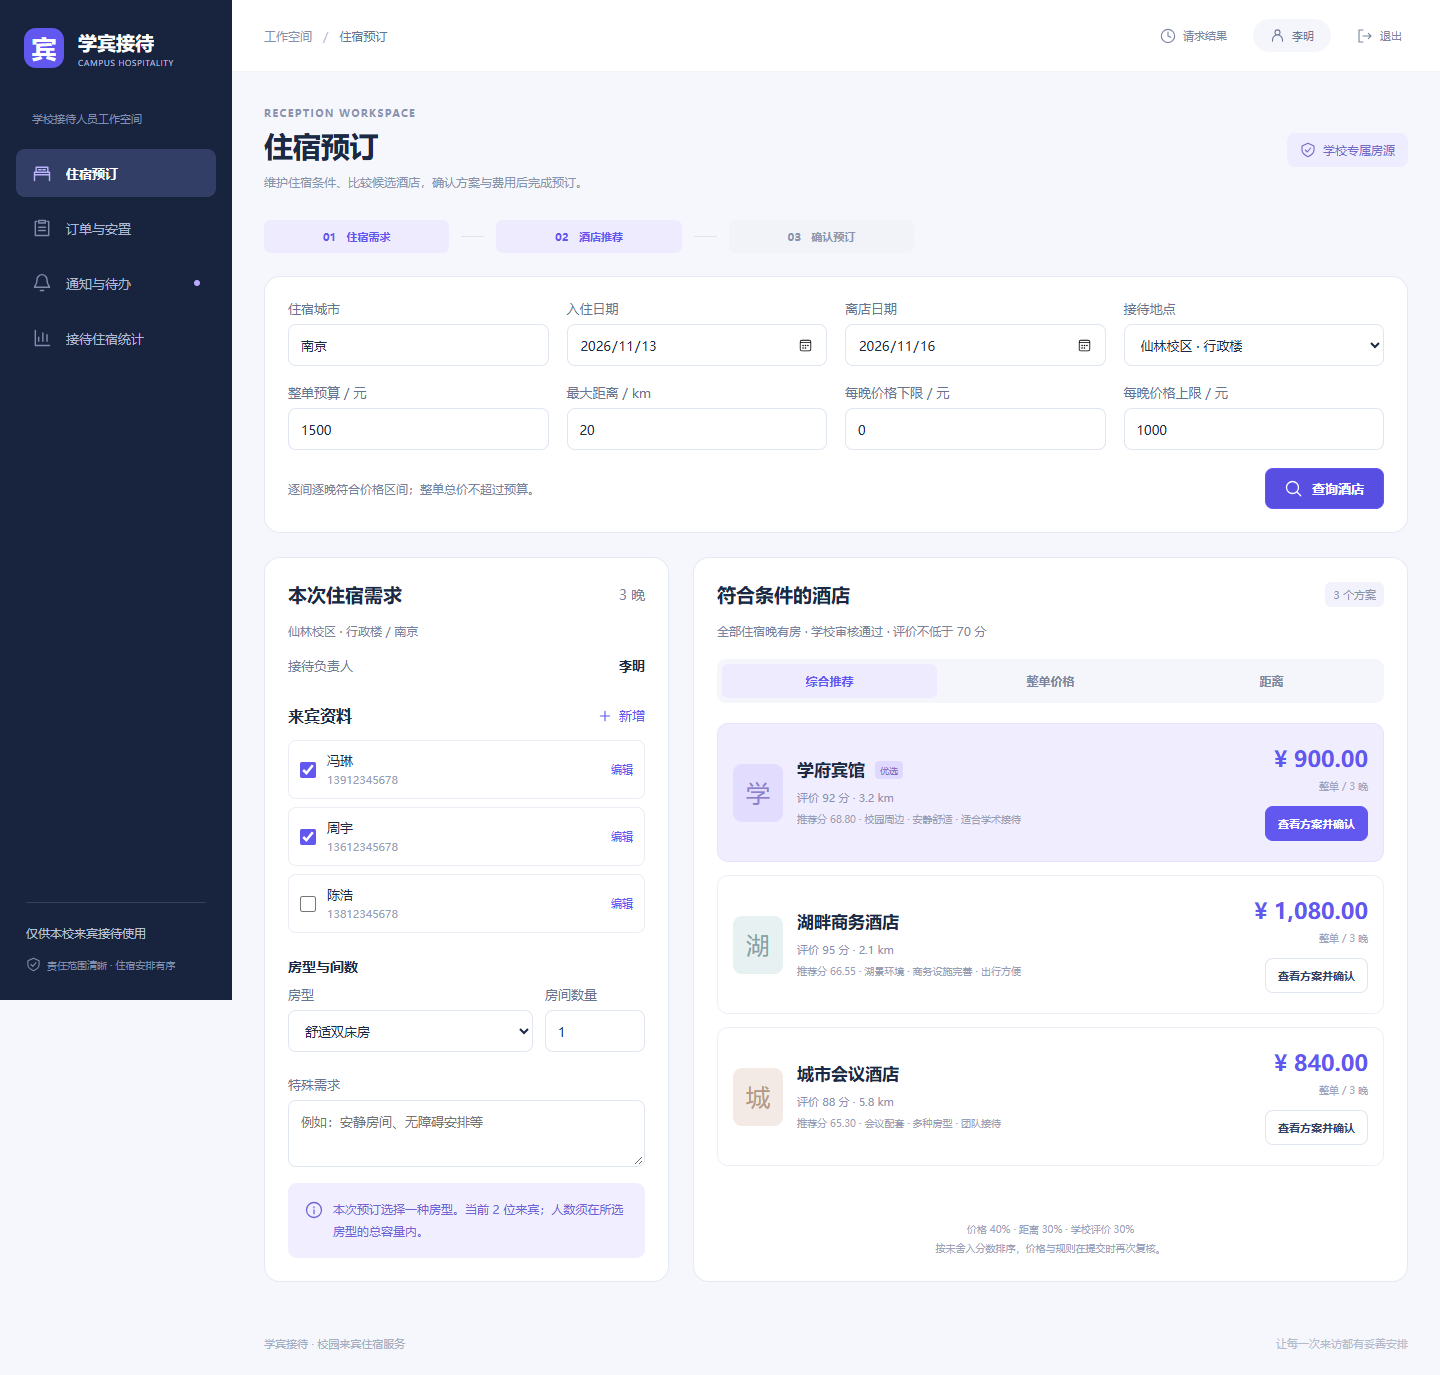
\includegraphics[width=\linewidth,height=157mm,keepaspectratio]{code/docs/screenshots/reception.png}
  \caption{接待人员查询酒店的实际运行界面（演示数据）}
  \label{fig:reception}
\end{figure}

并发争抢最后一间房时，测试中仅一笔预订成功。重复提交同一请求只创建一笔订单。改订目标房源不足时，保留原订单及名额占用。应用进程终止并重新启动后，抽查的 4 笔订单、93 条逐日房源和 1 条原请求终态结果均与重启前一致。以上为本地功能与持久性验证，生产 MySQL 环境、真实学校邮件及规定负载下的性能尚待验收。

\clearpage

\section{Git 远程代码管理展示}
\subsection{仓库与远程分支}

本次实验在项目目录初始化 Git 仓库，使用 \texttt{main} 分支，将远程 \texttt{origin} 配置为实验三仓库。首次提交共纳入 129 个文件，包含 \path{code/} 下的源码、配置模板、测试及构建脚本，以及需求、架构、UML 图、UI 原型和代码风格检查清单。\href{https://github.com/wsyheqi/software_engineering_task3}{GitHub 实验三仓库}

\path{.gitignore} 将本机数据库、运行日志、依赖目录、构建缓存、发布包和本机启动快捷方式排除在版本控制之外。软件可通过仓库中的构建脚本重新打包。

\subsection{实现提交与远程核对}

2026 年 11 月 24 日，我将实现提交 \texttt{efdbf1a} 推送至 GitHub，并让本地 \texttt{main} 跟踪 \texttt{origin/main}。首次推送和随后查询远程分支时得到以下记录。\href{https://github.com/wsyheqi/software_engineering_task3/commit/efdbf1a3d0a81ba7344da5d6f7751d989b4b9c23}{查看实现提交}

{\small
\begin{verbatim}
$ git push --set-upstream origin main
To https://github.com/wsyheqi/software_engineering_task3.git
 * [new branch]      main -> main
branch 'main' set up to track 'origin/main'.

$ git ls-remote --symref origin HEAD refs/heads/main
ref: refs/heads/main                         HEAD
efdbf1a3d0a81ba7344da5d6f7751d989b4b9c23      HEAD
efdbf1a3d0a81ba7344da5d6f7751d989b4b9c23      refs/heads/main
\end{verbatim}
}

核对时，GitHub 的默认分支为 \texttt{main}，远程返回的完整编号与本地实现提交一致。实验报告的 LaTeX 源文件和 PDF 在实现提交之后单独提交，报告内的提交编号可以定位本次实验的代码版本。\href{https://github.com/wsyheqi/software_engineering_task3/commits/main/}{查看分支提交历史}

\end{document}
